\documentclass[10pt]{beamer}

\usepackage[utf8]{inputenc}
\usepackage[spanish]{babel}
\usepackage{graphicx}

\mode<presentation>
\usetheme{Madrid}
%\usecolortheme[RGB={111,73,135}]{structure}
\usecolortheme[RGB={128,0,0}]{structure}
%\usecolortheme[RGB={0,96,0}]{structure}
%\usecolortheme[RGB={200,0,200}]{structure}
%\usecolortheme[RGB={0,128,0}]{structure}
%\usecolortheme[RGB={0,0,128}]{structure}
\usefonttheme{serif}
\useinnertheme{rectangles}
\useoutertheme{split}
\setbeamercovered{transparent}


% Definiciones para usar luego
\newtheorem{ejemplo}{Ejemplo}
\newtheorem{definicion}{Definición}

\title{Entendiendo y Optimizando MySQL}
\author{Jesús Espino García}
\date{10 de Noviembre de 2010}
\subject{Entendiendo y Optmizando MySQL}

\institute[GUL UC3M]{
  Grupo de Usuarios de Linux\\
  Universidad Carlos III de Madrid.\\
  \ \\
  
\includegraphics[height=1.5cm]{imgs/gul}}

\setcounter{tocdepth}{2}

\AtBeginSubsection[]
{
  \begin{frame}<beamer>{Indice}
    \tableofcontents[sectionstyle=show/shaded,subsectionstyle=show/shaded/hide]
  \end{frame}
}

\begin{document}

  \frame{\maketitle}
  
  \section{Introducción}

\subsection{Introducción}
\begin{frame}{Introducción}
  \begin{itemize}
    \item Sistema de Gestion de Bases de Datos.
    \item Software Libre.
    \item GPL.
    \item Escrito en C y C++
    \item Multiplataforma
    \item Mas de 6 millones de instalaciones.
  \end{itemize}
\end{frame}

\subsection{Arquitectura}
\begin{frame}{Arquitectura}
  \begin{center}
    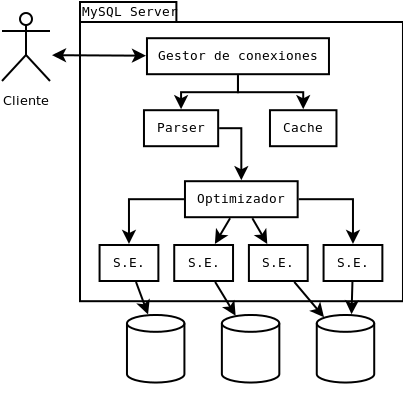
\includegraphics[height=5.5cm]{imgs/arch.png}
  \end{center}
\end{frame}

  \section{Esquemas e índices}

\subsection{Introducción}
\begin{frame}{Introducción}
  \begin{itemize}
    \item Nuestros esquemas e índices dependen de la funcionalidad.
    \item Es tan importante el que, como el como.
    \item Todo el diseño debe tener en cuenta los casos de uso.
    \item Es muy diferente un diseño para lectura, escritura o baja latencia.
    \item Todo deriva en un compromiso entre el rendimiento en diferentes situaciones.
  \end{itemize}
\end{frame}

\subsection{Normalización}
\begin{frame}{Normalización}
  \begin{itemize}
    \item Reestructuración de nuestras tablas.
    \item Busca eliminar redundancia.
    \item Se aplican una serie de ''formas normales''.
    \item Normalmente es una buena política.
  \end{itemize}
\end{frame}

\begin{frame}{Des-normalización}
  \begin{itemize}
    \item A veces la normalización es ineficiente.
    \item La redundancia puede producir incrementos de rendimiento significativos.
    \item Bases de datos con mucha lectura y poca escritura.
    \item Bases de datos con necesidades de latencias muy bajas.
  \end{itemize}
\end{frame}

%\subsection{Filas de tamaño fijo}
%\begin{frame}{Filas de tamaño fijo}
%  \begin{itemize}
%    \item Las filas almacenadas en nuestra base de datos tienen un tamaño.
%    \item Este puede ser fijo o variable.
%    \item Las filas de tamaño fijo son mas rápidas.
%    \item Una fila se considera de tamaño fijo, si todos sus campos lo son.
%    \item A veces conviene desaprovechar cierta cantidad de espacio a cambio de rendimiento.
%    \item Dependiendo del tipo de consulta puede resultar mas rápido si ahorramos espacio.
%  \end{itemize}
%\end{frame}

\subsection{Índices}
\begin{frame}{Índices}
  \begin{itemize}
    \item Estructuras auxiliares para búsquedas.
    \item Aceleran las consultas (cuando tienen datos suficientes).
    \item Pueden resolver la consulta entera (si los datos necesarios están contenidos).
    \item Hacen referencia a uno o mas campos.
    \item Los índices de varios campos tienen un orden concreto.
    \item (A,B) != (B,A)
    \item Cada índice incrementa el espacio consumido y decrementa la velocidad de escritura.
  \end{itemize}
\end{frame}

\begin{frame}{Arboles B}
  \begin{itemize}
    \item Este es tipo de índice mas habitual.
    \item El formato interno del árbol depende del S.E.
    \item Este tipo de índice permite las siguientes consultas:
    \begin{itemize}
      \item El valor completo del índice.
      \item Valores en la parte izquierda del índice.
      \item Rangos de valores.
      \item Una parte exacta (a la izquierda), y el resto como un rango.
      \item Consultas de solo el índice.
    \end{itemize}
  \end{itemize}
\end{frame}

\begin{frame}{Tablas hash}
  \begin{itemize}
    \item Para cada columna, se calcula un hash y se asocia al índice.
    \item Solo permite búsquedas exactas.
    \item Las búsquedas son muy rápidas.
    \item Es el tipo por defecto del S.E. Memory.
    \item Este modo no esta disponible en MyISAM o InnoDB, pero se puede ''emular''.
  \end{itemize}
\end{frame}

\begin{frame}{Spatial indexes}
  \begin{itemize}
    \item Índices especiales para GIS.
  \end{itemize}
\end{frame}

\begin{frame}{Full text}
  \begin{itemize}
    \item Índices para búsquedas sobre el contenido.
    \item Solo disponibles en MyISAM (por ahora).
  \end{itemize}
\end{frame}

\begin{frame}{Clustered indexes}
  \begin{itemize}
    \item No es otro tipo de índice, es un concepto.
    \item Consiste en incluir los datos de la fila, dentro del índice de la clave primaria.
    \item Esto permite que la búsqueda de la clave primaria de como resultado la fila, sin necesidad de ningún salto extra.
    \item InnoDB implementa este tipo de árbol B.
  \end{itemize}
\end{frame}

\begin{frame}{Coverage indexes}
  \begin{itemize}
    \item Extraer los datos directamente del índice.
    \item Solo si todos los datos están contenidos en el índice.
    \item Supone un incremento significativo del rendimiento.
  \end{itemize}
\end{frame}

  \section{Componentes}
\subsection{El servidor}
\begin{frame}{El servidor}
  \begin{itemize}
    \item Espera las conexiones de los usuarios.
    \item Hace la validacion.
    \item Comprueba si la consulta esta en la cache.
    \item Si la consulta esta en la cache, devuelve el resultado.
    \item Si la consulta no esta en la cache, la pasa al parser.
    \item 
  \end{itemize}
\end{frame}

\subsection{La cache}
\begin{frame}{La cache}
  \begin{itemize}
    \item La cache almacena resultados asociados a "hash" de consultas.
    \item Cualquier modificacion en una tabla relacionada con una consulta, caduca esa consulta en la cache.
    \item 
    \item 
  \end{itemize}
\end{frame}

\subsection{El parser}
\begin{frame}{El parser}
  \begin{itemize}
    \item Recibe una consulta en SQL, y la convierte en una estructura de arbol.
    \item Se preprocesa el arbol y hace cambios que el parser no hace.
    \item Pasa la estructura de arbol al optimizador.
  \end{itemize}
\end{frame}

\subsection{El optimizador}
\begin{frame}{El optimizador}
  \begin{itemize}
    \item Utiliza la estructura de arbol para hacer optimizaciones.
    \item Mediante datos estadisticos del S.E. y algoritmos de optimizacion hace diferentes pruebas.
    \item Escoje la prueba que le haya dado un valor mas optimo.
    \item Algunos ejemplos de algoritmos de optimizacion:
    \begin{itemize}
      \item Reordenacion de Joins
      \item Aplicacion de reglas algebraicas.
      \item Evaluacion y reduccion de expresiones constantes.
      \item \dots
    \end{itemize}
    \item Como resultado del optimizador se optine el "execution plan" que se aplica a los S.E.
  \end{itemize}
\end{frame}

\subsection{Storage Engines}
\begin{frame}{Introducción}
  \begin{itemize}
    \item Recibe peticiones simples de acceso a datos.
    \item Mediante estas operaciones simples se satisface el "execution plan".
    \item Cada S.E. tiene funcionalidades y capacidades diferentes.
    \item 
    \item 
  \end{itemize}
\end{frame}

\begin{frame}{MyISAM}
  \begin{itemize}
    \item El tipo por defecto de MySQL.
    \item Muy rapido
    \item Lock por tablas
    \item Indices B-Tree y Full-Text
    \item Tablas comprimidas (solo lectura)
  \end{itemize}
\end{frame}

\begin{frame}{InnoDB}
  \begin{itemize}
    \item Transaccional (ACID).
    \item Lock por filas.
    \item Integridad referencial.
    \item Indices B+Tree con clustered index.
  \end{itemize}
\end{frame}

\begin{frame}{Memory (Heap)}
  \begin{itemize}
    \item Tablas en memoria.
    \item Muy rapidas.
    \item Se pierden todos los datos al reiniciar el mysql.
    \item Indices Hash y B-Tree.
  \end{itemize}
\end{frame}

\begin{frame}{CSV}
  \begin{itemize}
    \item Lock por tabla.
    \item Gestiona los datos como ficheros csv.
    \item Util para gestionar datos compartidos con otras aplicaciones que solo entienden CSV.
  \end{itemize}
\end{frame}

\begin{frame}{BlackHole}
  \begin{itemize}
    \item Transaccional (ACID).
    \item Lock por filas.
    \item Descarta cualquier insert.
    \item El sistema de logs sigue funcionando.
  \end{itemize}
\end{frame}

\begin{frame}{Archive}
  \begin{itemize}
    \item Transaccional (ACID).
    \item Lock por filas.
    \item Base de datos orientada a escritura.
    \item Ideal para almacenar logs.
  \end{itemize}
\end{frame}

\begin{frame}{Federated}
  \begin{itemize}
    \item Tabla virtual, traduce las consultas a consultas DBMS.
  \end{itemize}
\end{frame}

\begin{frame}{Otros}
  \begin{itemize}
    \item Maria
    \item BerkeleyDB
    \item Merge
    \item NDB
    \item Falcon
    \item \dots
  \end{itemize}
\end{frame}

  \section{Las queries}

\subsection{Las queries}
\begin{frame}{Las queries}
  \begin{itemize}
    \item 
    \item 
    \item 
    \item 
  \end{itemize}
\end{frame}

  \section{Escalando MySQL}

\subsection{Escalado vertical}
\begin{frame}{Escalado vertical}
  \begin{itemize}
    \item Ampliar o mejorar el hardware.
    \item MySQL no se adapta muy bien al escalado vertical.
    \item Depende mucho del tipo de uso que se haga del mysql.
  \end{itemize}
\end{frame}

\subsection{Escalado horizontal}
\begin{frame}{Escalado horizontal}
  \begin{itemize}
    \item Distribucion de los datos.
    \item Varias opciones:
    \begin{itemize}
      \item Replicacion (y uso de los esclavos para lectura).
      \item Distribucion (por clave)
      \item Distribucion (por funcionalidad)
      \item Combinacion de las anteriores.
    \end{itemize}
  \end{itemize}
\end{frame}

\subsection{Escalado hacia atras}
\begin{frame}{Escalado hacia atras}
  \begin{itemize}
    \item Eliminacion de datos ya no necesarios.
    \item Datos de caracter historico que pueden ser eliminados o migrados.
  \end{itemize}
\end{frame}

\subsection{Escalado con cluster}
\begin{frame}{Escalado con cluster}
  \begin{itemize}
    \item MySQL Cluster es una implementacion de distribucion de datos transparente.
    \item Distribuye los datos entre un conjunto de nodos.
    \item Da buen rendimiento para consultas simples y pocos datos.
    \item Se comporta mal con consultas complejas y que requieran comunicacion entre nodos.
  \end{itemize}
\end{frame}

  \section*{Para terminar}
\subsection*{Otra información útil}
\begin{frame}{Referencias}
  \begin{itemize}
    \item Manual oficial de mysql (mysql.com).
    \item O'Reilly - High Performance MySQL (Second Edition).
    \item Apress - Pro MySQL.
  \end{itemize}
\end{frame}

\subsection*{Cierre}

\begin{frame}{¿Qué queda en el tintero?}
  \begin{itemize}
    \item Alta disponibilidad
    \item Replicación
    \item Optimizaciones de configuración.
    \item Optimizaciones de SSOO.
    \item Optimizaciones de Hardware.
    \item \dots
  \end{itemize}
\end{frame}

\begin{frame}{Dudas}
  \begin{center}
    \dots
  \end{center}
\end{frame}

\begin{frame}{Fin}
  \begin{center}
    Gracias por venir.
  \end{center}
\end{frame}


\end{document}
